% !TEX program = xelatex

\documentclass[12pt,a4paper]{article}
\usepackage[UTF8]{ctex}
\usepackage{float}
\usepackage{amsmath}
\usepackage{enumerate}
\usepackage{booktabs}
\usepackage{graphicx}
\usepackage{longtable}
\usepackage{subfigure}

\usepackage{url}

% for plotting 
\usepackage{caption}
\usepackage{pgfplots}

% for pseudo code 
\usepackage{algorithm}
\usepackage[noend]{algpseudocode}

% for reference 
\usepackage{hyperref}
\usepackage{cleveref}

% for code 
\usepackage{listings}
\usepackage{xcolor}
\usepackage{fontspec}

% Microsoft Word A4 paper default layout 
\usepackage[a4paper, left=3.18cm, right=3.18cm, top=2.54cm, bottom=2.54cm]{geometry}

\title{DIP Lab 1: Point Processing}
\author{2017011620 计73 李家昊}
\date{\today}

\begin{document}

\captionsetup[figure]{labelfont={bf}, name={Figure}}
\captionsetup[table]{labelfont={bf}, name={Table}}

\maketitle

\section{Histogram Equalization}

\begin{figure}[H]
    \centering
    \subfigure[Original]{
        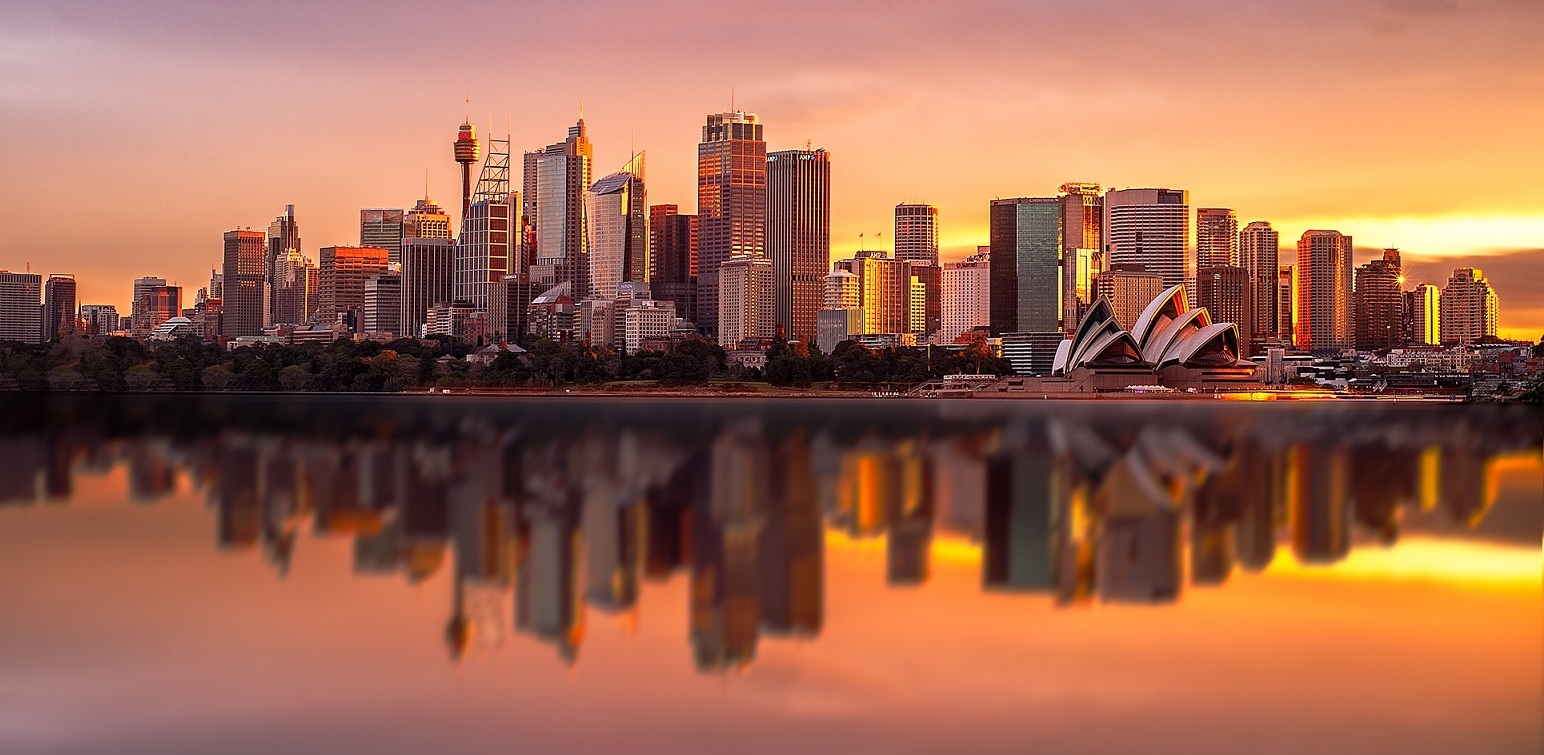
\includegraphics[width=0.95\textwidth]{../fig/sydney.jpg}
    }
    \subfigure[Output]{
        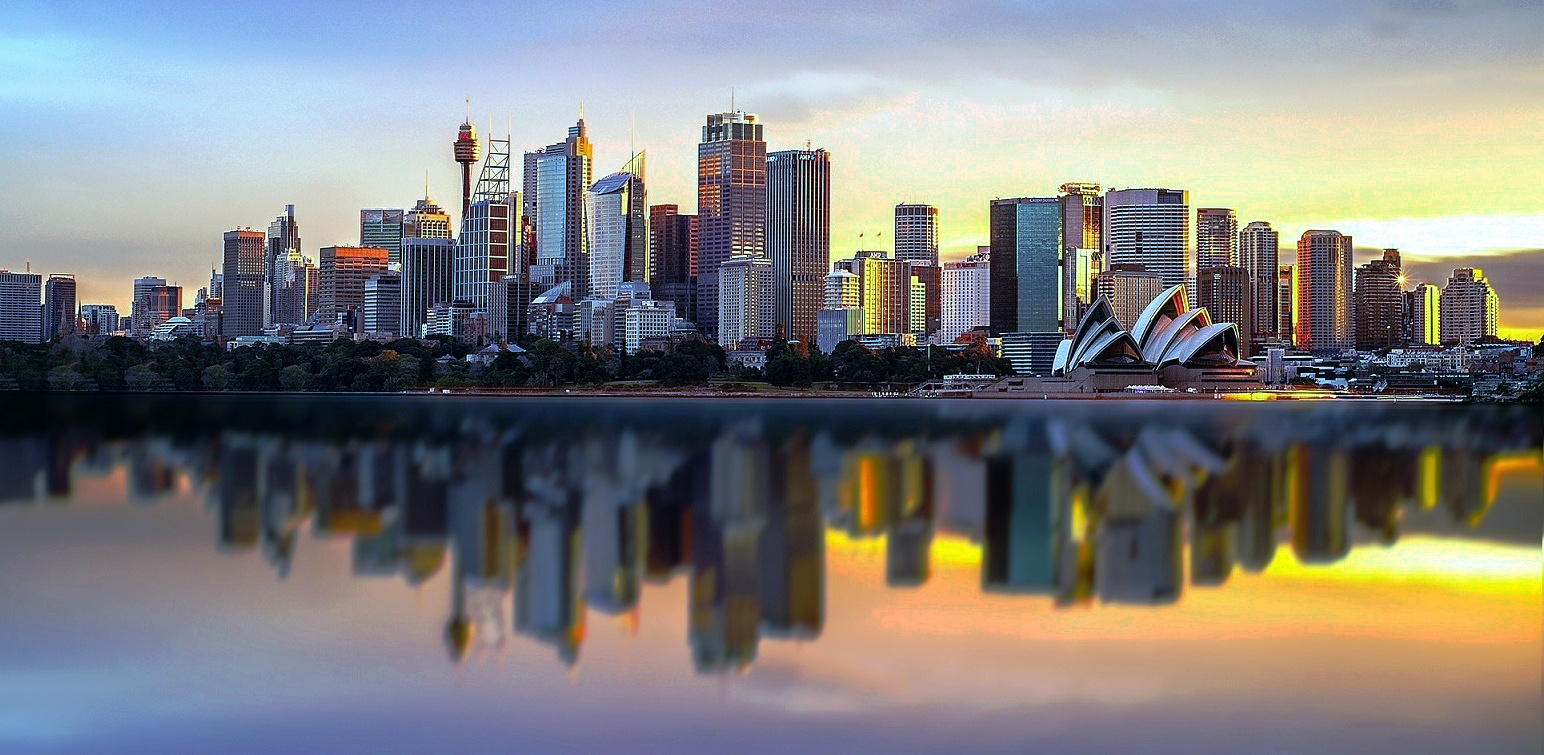
\includegraphics[width=0.95\textwidth]{../output/hist_eq.jpg}
    }
    \caption{Histogram Equalization}
    \label{fig:hist_eq}
\end{figure}

如\Cref{fig:hist_eq}所示,原图偏暖色调,为了使其色调更加均衡,这里在其三个channel上分别做直方图均衡化,每个channel上的LUT定义如下,
\begin{equation}
    \boldsymbol{J}(r, c) = 255 \cdot P(\boldsymbol{I}(r, c))
\end{equation}
其中$\boldsymbol{I}, \boldsymbol{J}$分别为输入和输出图像,$r, c$为行列坐标,$P(x)$为输入图像的CDF。

\section{Histogram Matching}

\begin{figure}[H]
    \centering
    \subfigure[Original]{
        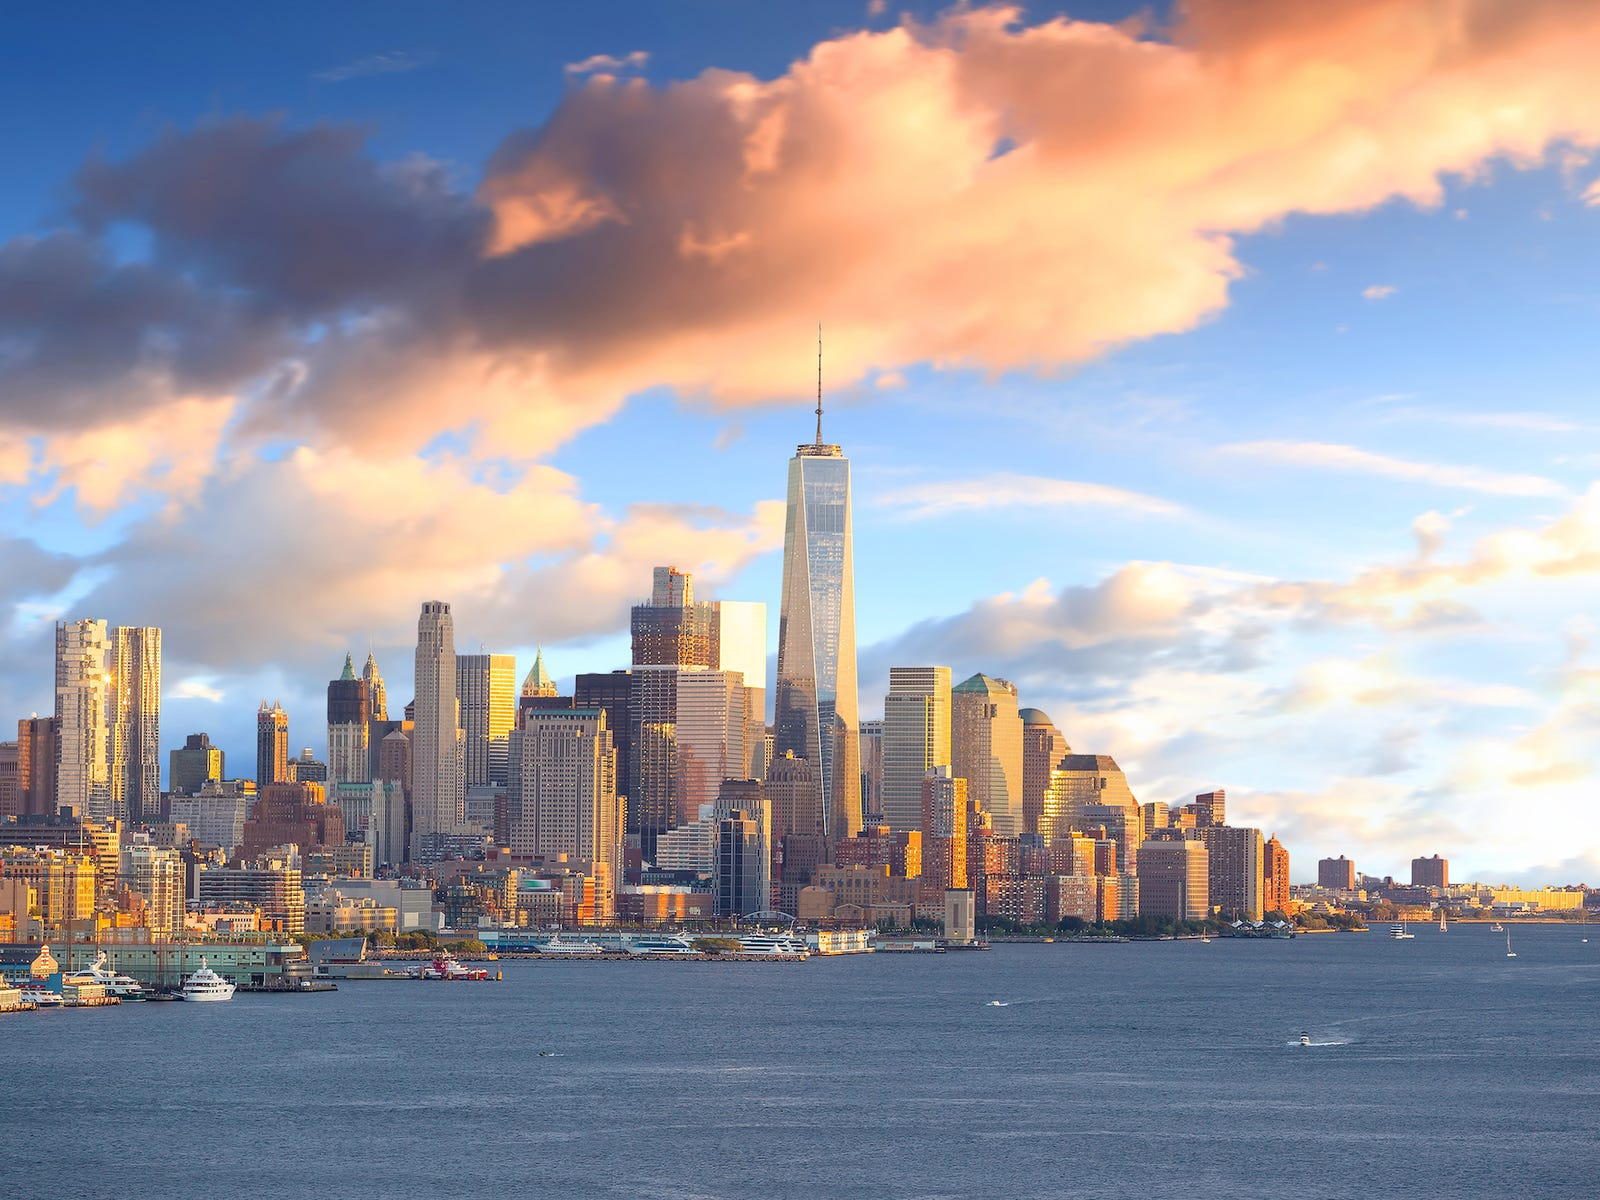
\includegraphics[width=0.47\textwidth]{../fig/new_york.jpg}
    }
    \subfigure[Target]{
        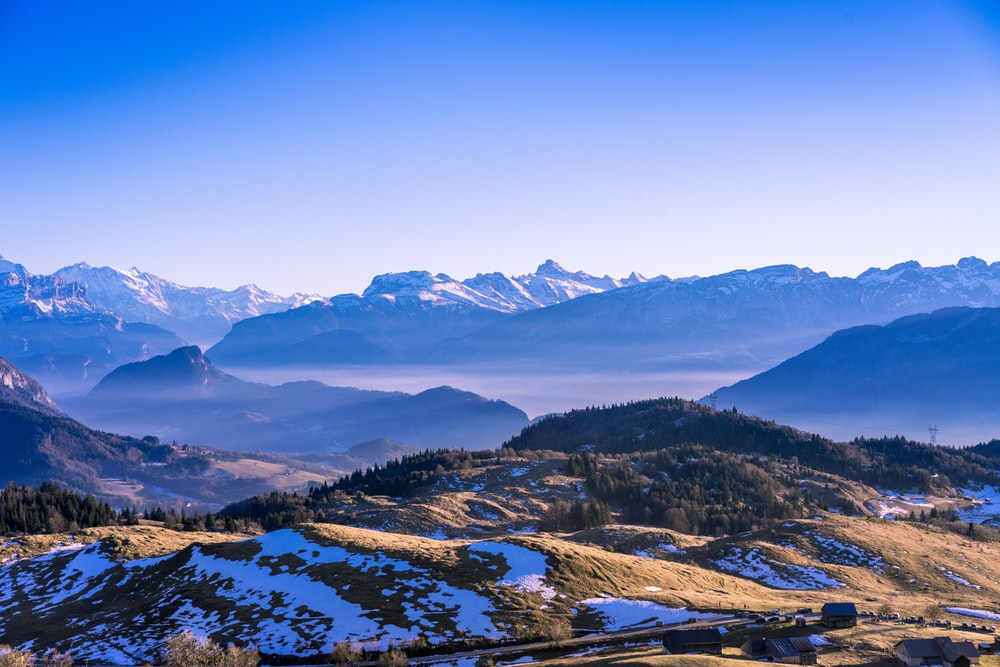
\includegraphics[width=0.47\textwidth]{../fig/scenery.jpg}
    }
    \subfigure[Output]{
        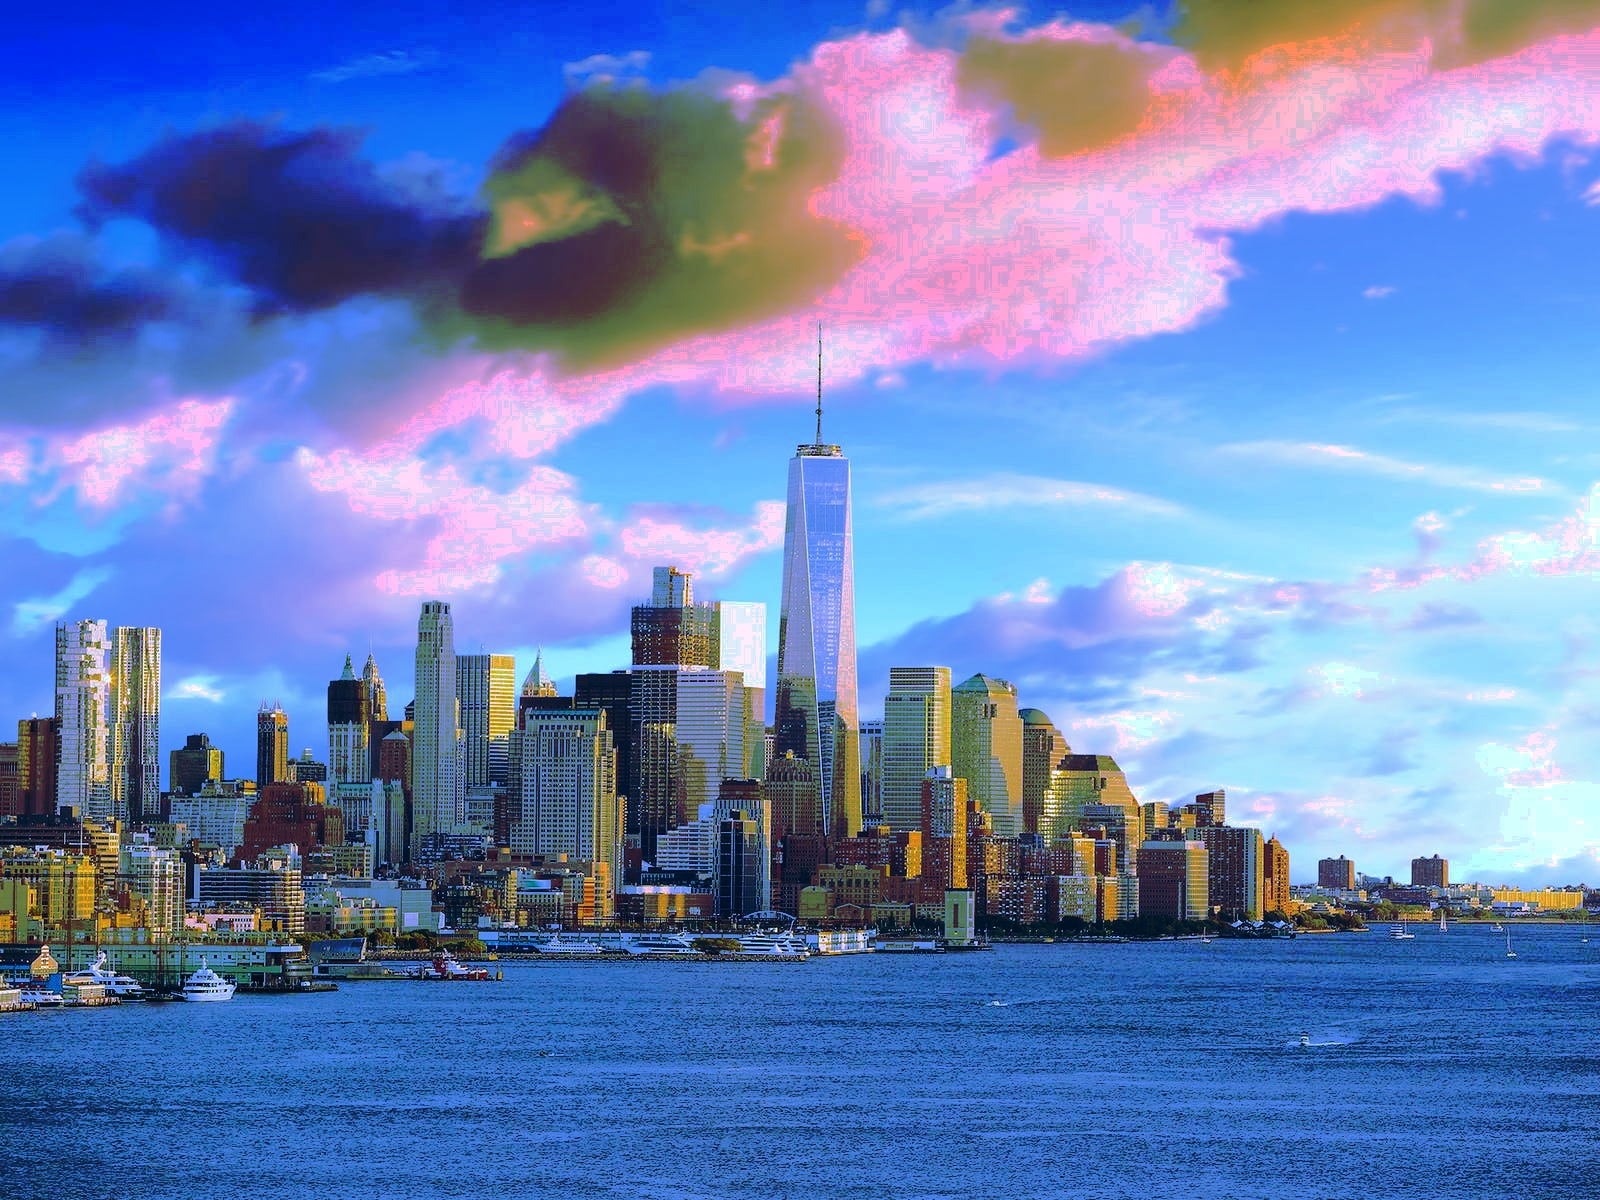
\includegraphics[width=0.7\textwidth]{../output/hist_match.jpg}
    }
    \caption{Histogram Matching}
    \label{fig:hist_match}
\end{figure}

如\Cref{fig:hist_match}所示,这里希望将原图的色调变成目标图像的色调,因此采用直方图匹配的方式迁移色调,LUT定义如下,
\begin{equation}
    \boldsymbol{J}(r, c) = P_{T}^{-1} ( P_{I}(\boldsymbol{I}(r, c)))
\end{equation}
其中$P_T$为目标图像的CDF,$P_I$为输入图像的CDF。

\section{Contrast Enhancement}

\begin{figure}[H]
    \centering
    \subfigure[Original]{
        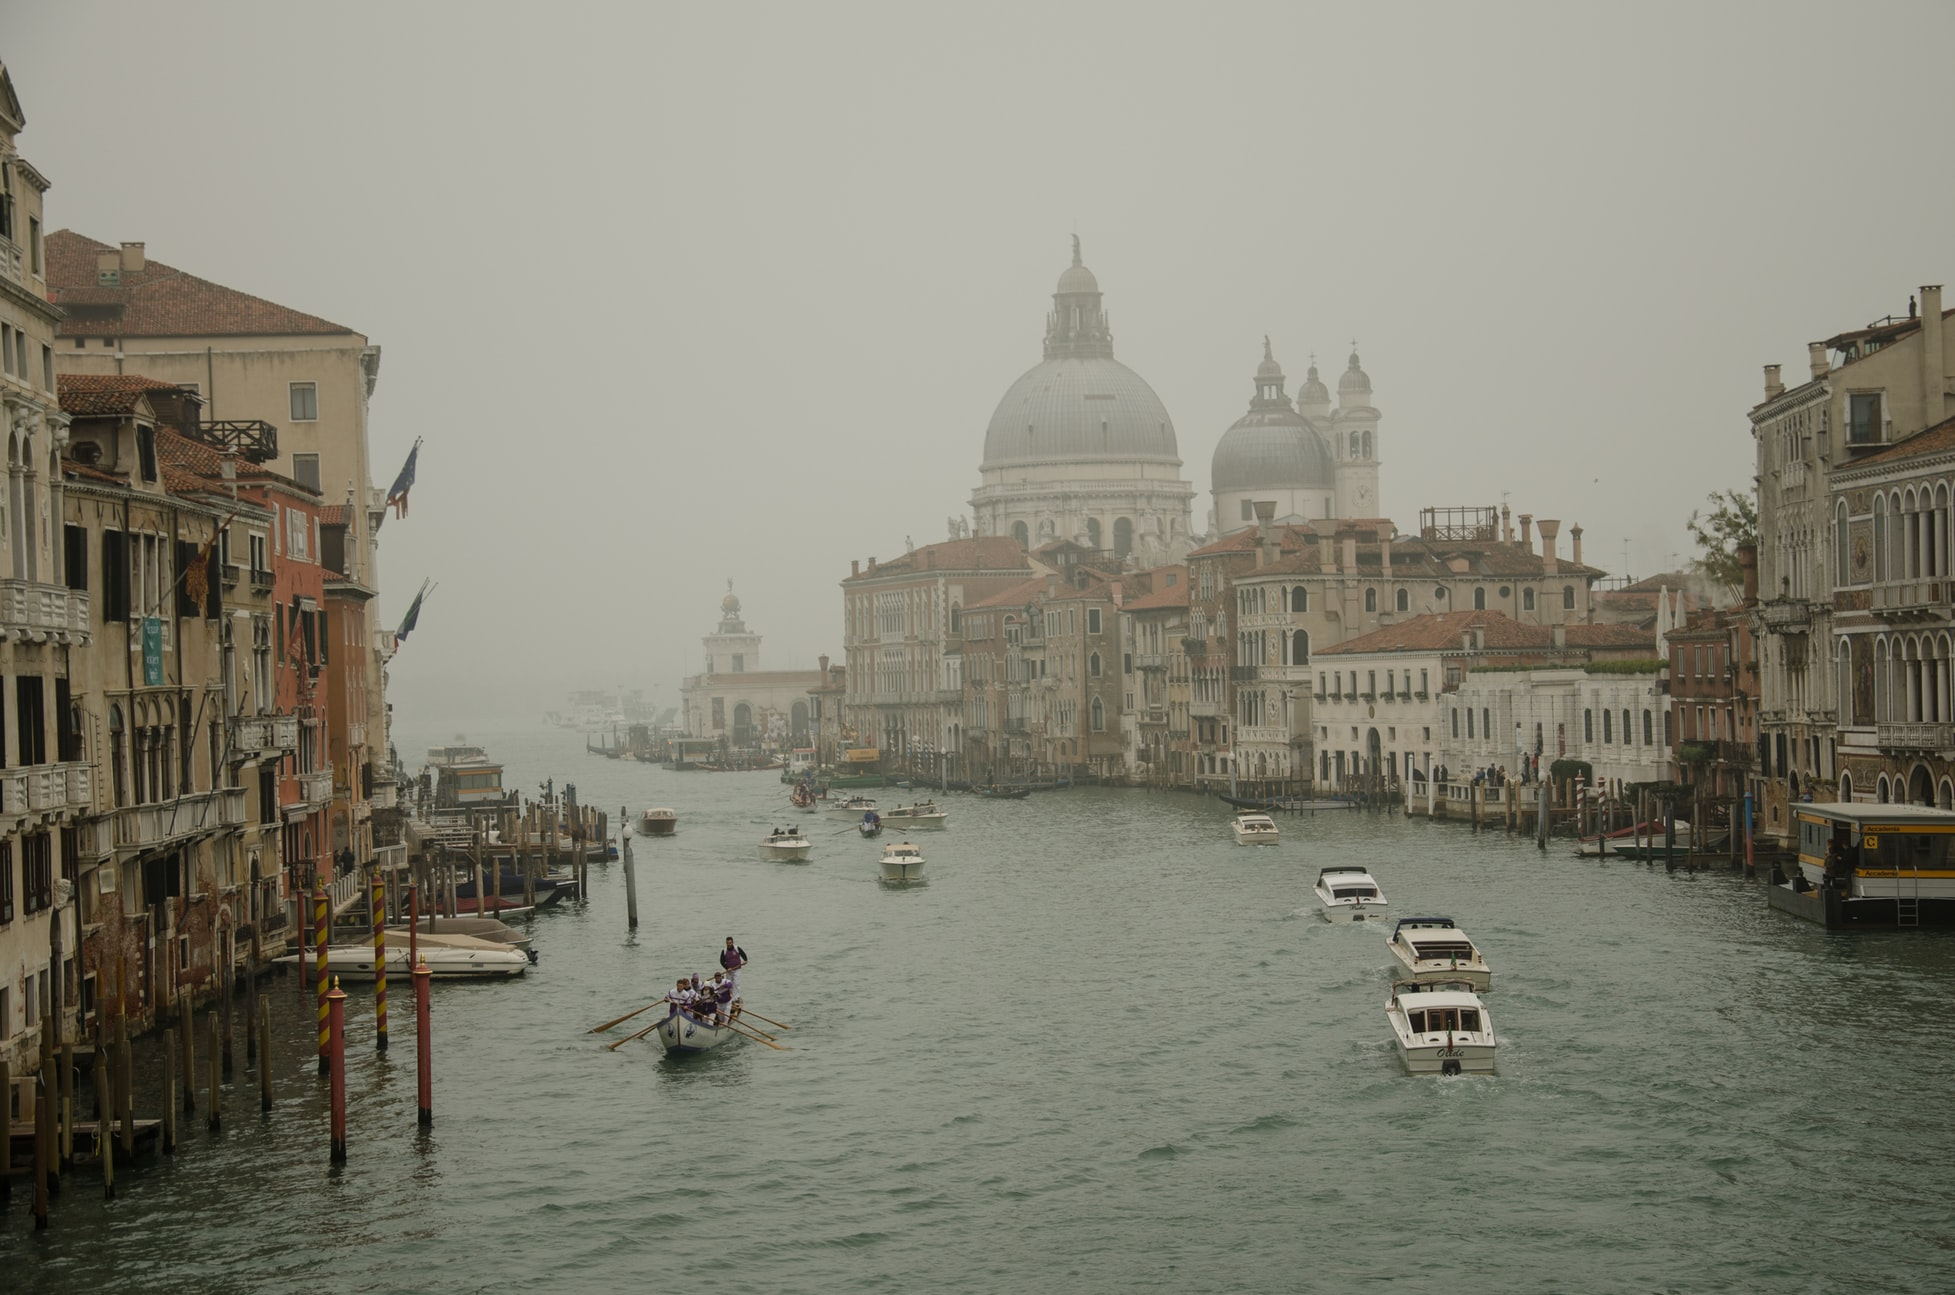
\includegraphics[width=0.9\textwidth]{../fig/venice.jpg}
    }
    \subfigure[Output]{
        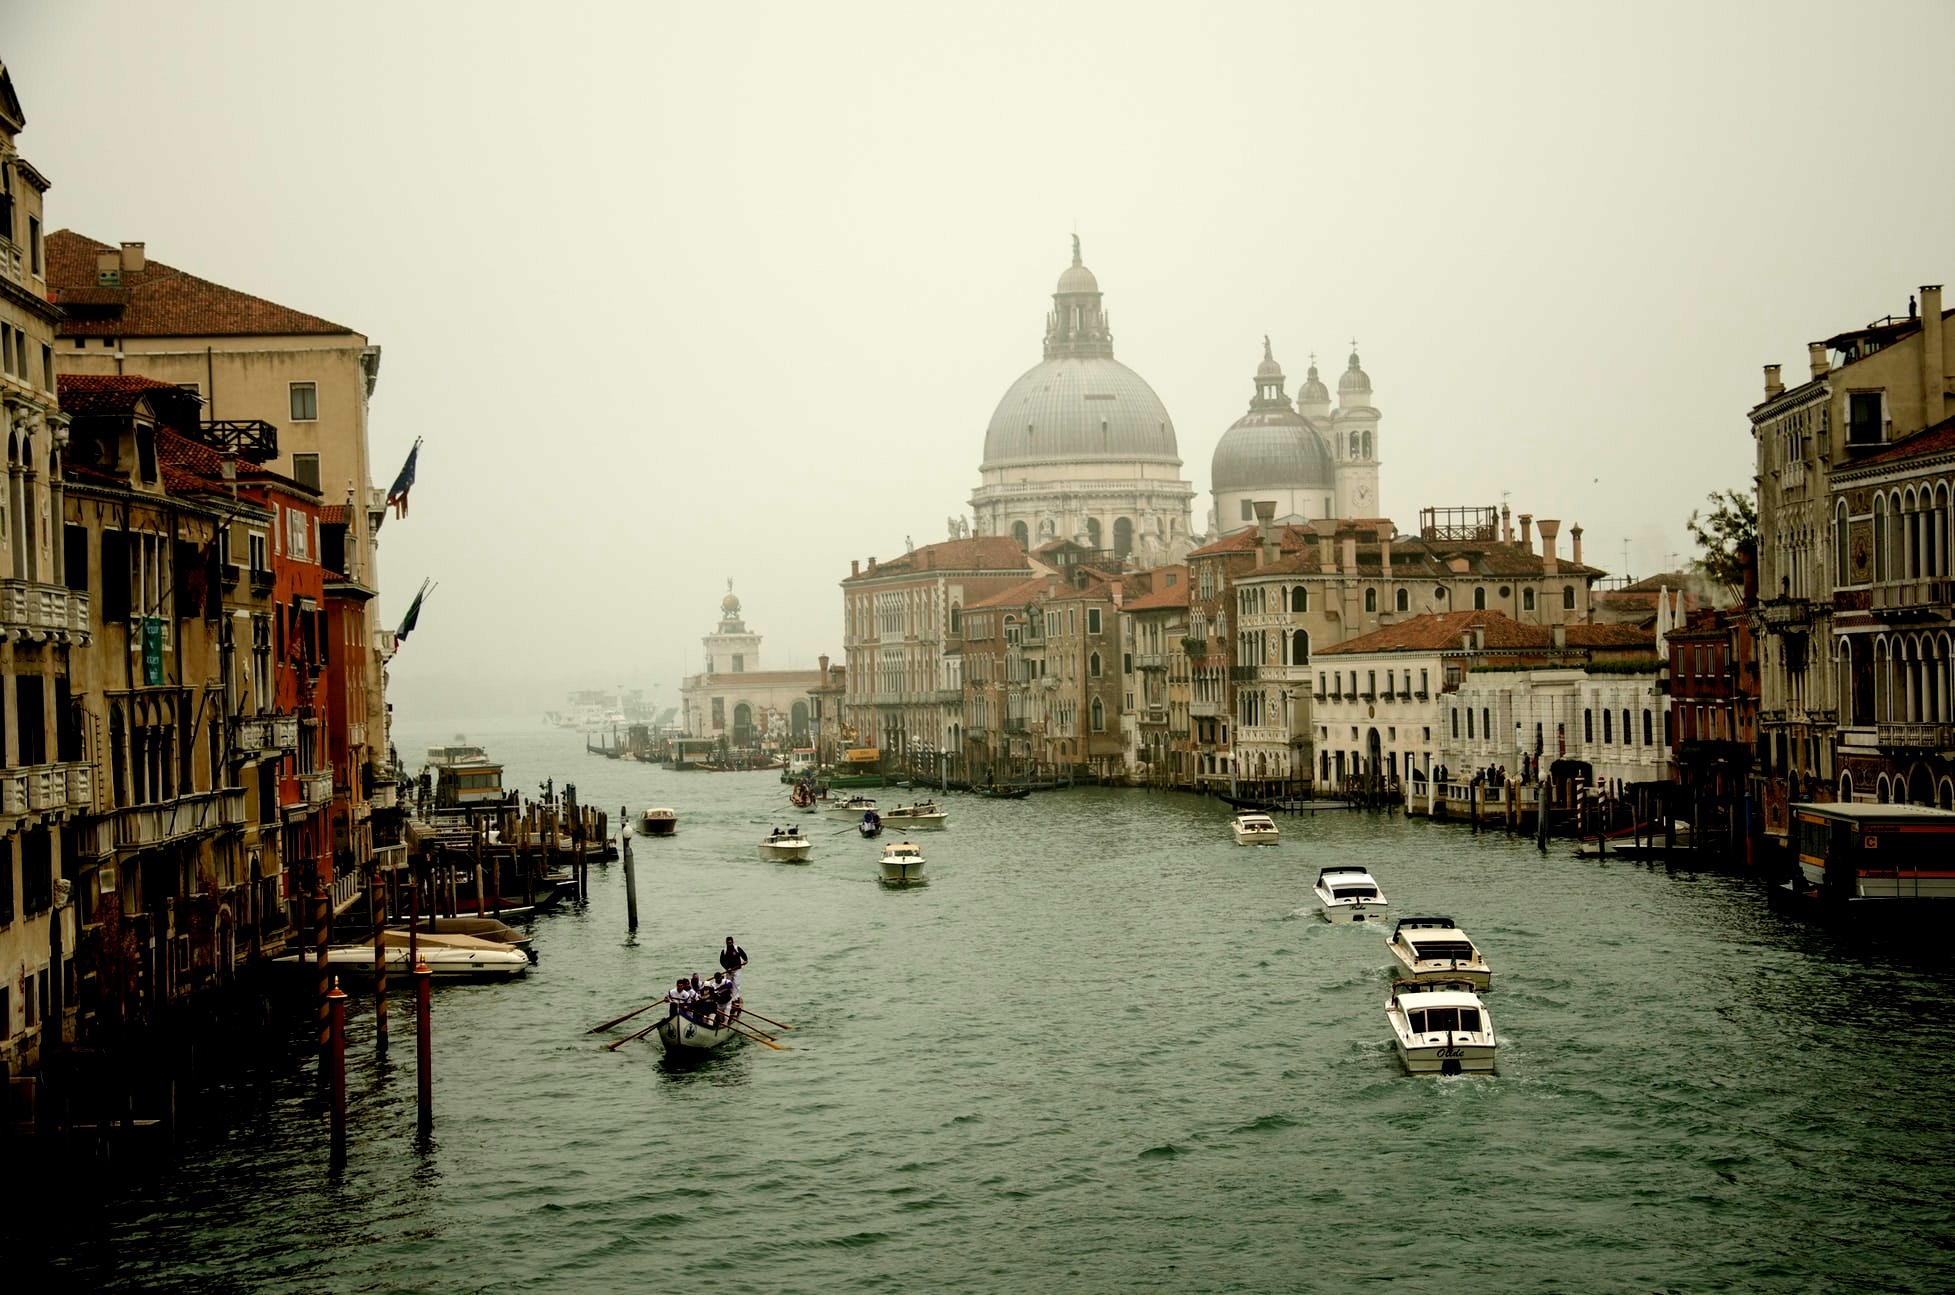
\includegraphics[width=0.9\textwidth]{../output/contrast.jpg}
    }
    \caption{Contrast Enhancement}
    \label{fig:contrast}
\end{figure}

如\Cref{fig:contrast}所示,原图有雾,故采用对比度增强的方式去雾,LUT定义为,
\begin{equation}
    \boldsymbol{J}(r, c) = a \left(\boldsymbol{I}(r, c) - 127\right) + 127
\end{equation}
其中设定系数$a=2$来增强对比度。

\section{Gamma Correction}

\begin{figure}[H]
    \centering
    \subfigure[Original]{
        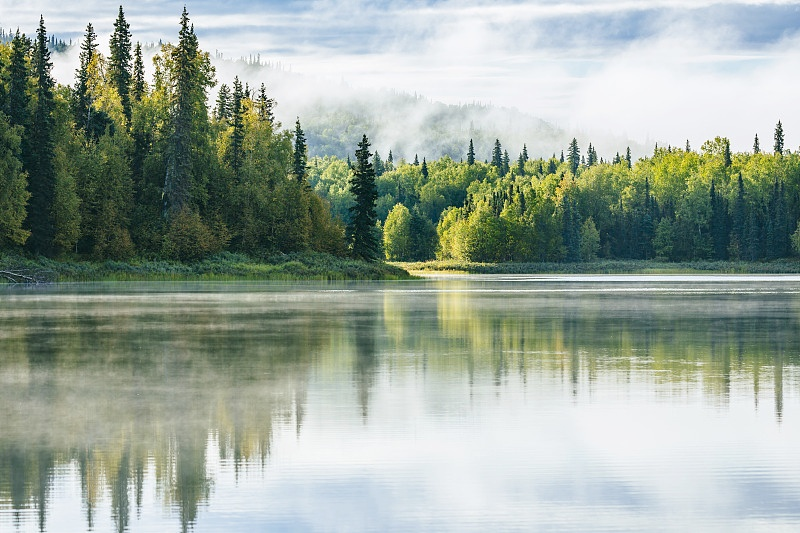
\includegraphics[width=0.85\textwidth]{../output/gamma_compression.jpg}
    }
    \subfigure[Output]{
        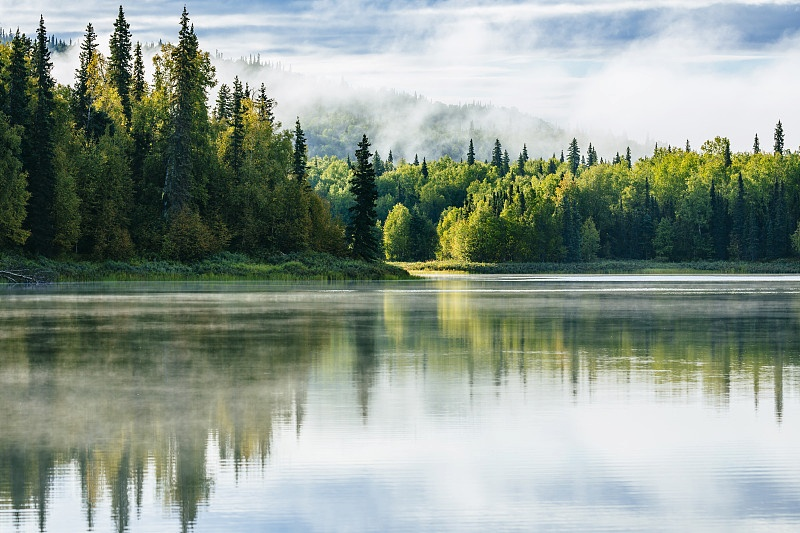
\includegraphics[width=0.85\textwidth]{../output/gamma_expansion.jpg}
    }
    \caption{Gamma Correction}
    \label{fig:gamma}
\end{figure}

如\Cref{fig:gamma}所示,原图总体亮度较高,层次感不强,考虑到人眼对暗处比较敏感,故采用Gamma校正将图片向暗处偏移,减少高光冗余,LUT如下,
\begin{equation}
    \boldsymbol{J}(r, c) = 255 \cdot \left(\frac{\boldsymbol{I}(r, c)}{255}\right)^\gamma
\end{equation}
其中取参数$\gamma=1.25$。


\section{Saturation Adjustment}


\begin{figure}[H]
    \centering
    \subfigure[Original]{
        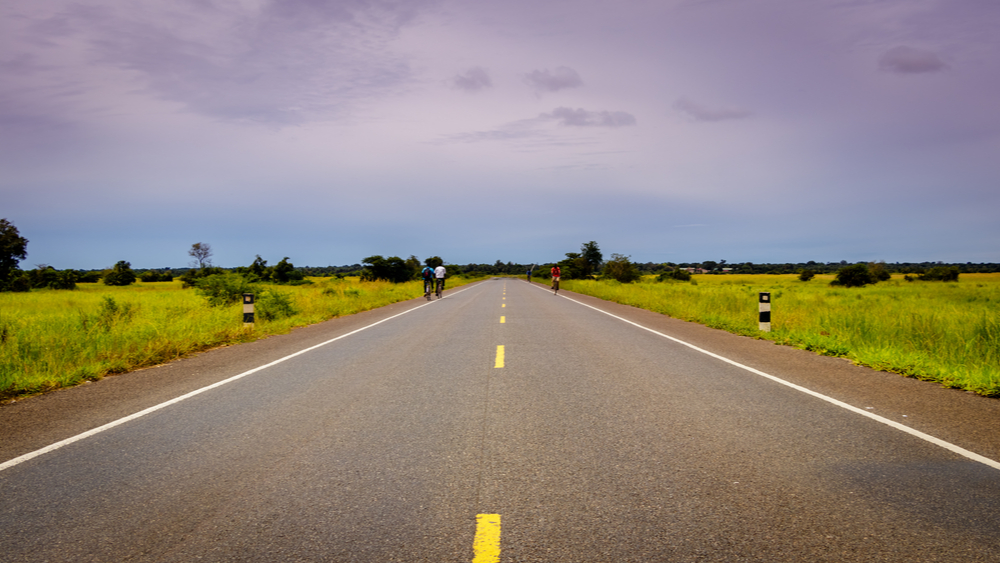
\includegraphics[width=0.95\textwidth]{../fig/road.jpg}
    }
    \subfigure[Output]{
        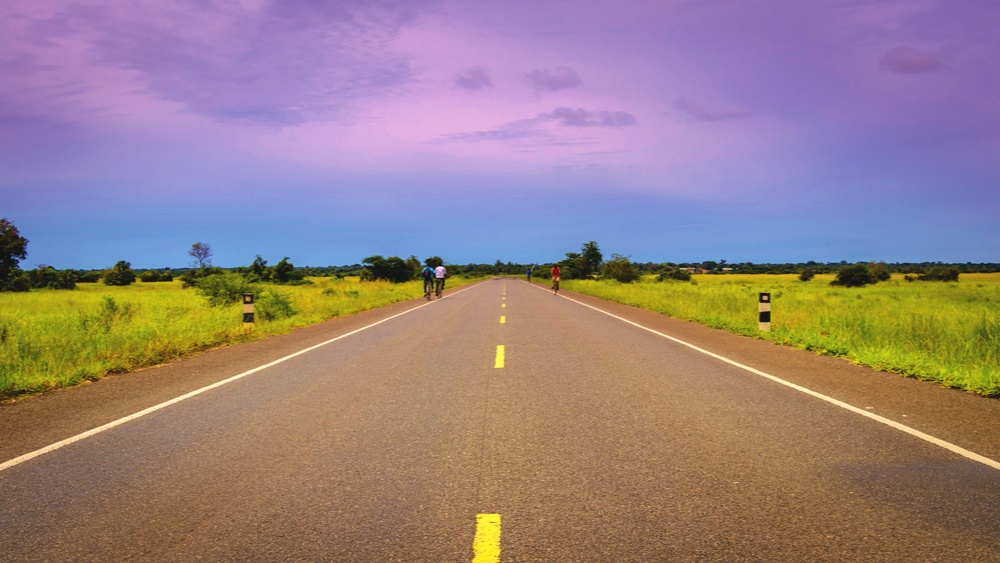
\includegraphics[width=0.95\textwidth]{../output/saturation.jpg}
    }
    \caption{Saturation Adjustment}
    \label{fig:saturation}
\end{figure}

如\Cref{fig:saturation}所示,为了使原图颜色更加饱满,这里尝试采用幂函数来调节饱和度,使用的LUT为,
\begin{equation}
    \boldsymbol{J}(r, c, b) =
    \begin{cases}
        255 \cdot \left(\dfrac{\boldsymbol{I}(r, c, b)}{255}\right)^\gamma, & b=1\\
        \boldsymbol{I}(r, c, b), & b\ne 1\\
    \end{cases}
\end{equation}
其中$\gamma=0.5$,输入输出图像均为HSV模式,$b=1$表示饱和度通道。

\section{遇到的问题}

本次作业的算法较为简单,实现上没有遇到什么困难。主要的问题是如何挑选合适的图片,以及采用哪种算法处理这些图片,使得它们更好看,这通常需要一些经验性的知识。

\end{document}
